\chapter*{Conclusion}
\addcontentsline{toc}{chapter}{Conclusion} % To add to TOC

\initial{I}t is now time to conclude this document, whose purpose was twofold:
exhibit clear theoretical properties of analogical classifiers, and apply
analogical inference to the field of recommender systems. Let us first recap
our main results and contributions (we will not necessarily follow the order of
the chapters here).

\paragraph{Contributions\\}

The first chapter was dedicated to give the necessary background on existing
models of analogical reasoning,  with a strong emphasis on models that allow
to build computer programs. In the second chapter, we thoroughly described
various definitions of analogical proportions in different settings, with a
particular focus on the arithmetic and the Boolean proportions. We have tried to
provide the reader with different geometrical insights on these proportions,
which were hopefully useful to gain a better intuition.
Finally, we considered a toy classification problem in a Boolean setting that
allowed us to introduce the analogical equation solving process and most
importantly, our analogical inference principle. This principle states that if
we have $a:b::c:d$, then we should also have $f(a) : f(b) :: f(c):f(d)$, where
$f(x)$ is the label of $x$, or any characteristic of interest.  When $f(d)$ is
unknown, it can be \textbf{inferred} from the values of $f(a)$, $f(b)$ and
$f(c)$, allowing us to apply this form of analogical reasoning to
classification tasks, or more general problems such as that of rating
prediction for recommendation tasks.\\

Analogical recommendation was addressed in Chapters
\ref{CHAP:background_reco_systems} and \ref{CHAP:analogical_recommendation}.
Chapter \ref{CHAP:background_reco_systems} was a background chapter, where we
clearly defined the problem we planned to address, and described two popular
collaborative filtering families (neighborhood methods and
matrix-factorization techniques) that will be compared to our custom algorithms
in the experiments.

We then developed in Chapter \ref{CHAP:analogical_recommendation} an algorithm
for rating prediction \cite{HugPraRicISMIS15}, on the basis that if four users
are in proportion (i.e. their respective ratings are in arithmetic proportion),
then it should also be the case for any item that one of the four users has not
rated. This approach is directly inspired from past works on analogical
classification. The experiments showed that this algorithm offers reasonable
performance compared to neighborhood techniques, but its cubic complexity makes
it simply impossible to use in real-world scenarios, due to enormous
computation time.

This led us to consider another kind of analogical recommendation, that does
not rely on the search of $3$-tuples of users. This ``clone''-based view
\cite{HugPraRicSerFuzzIEEE16} is motivated by the fact that some users may
have different interpretations of the rating scale that is used. Our results
show that the concept of ``clone'' is extremely relevant, but it must be noted
that this kind of bias in the user ratings had already been addressed in
previous works. As a side note, these works on the rating prediction task have
led us to build a Python library \cite{Surprise} that helps building and
analyzing such prediction algorithms.

Finally, we provided an algorithm for the mining of analogical proportions in
incomplete databases \cite{HugPraRicSerLFA16}, strongly inspired from the
mining of association rules. We used this algorithm to extract analogical
proportions between items in a rating database, which actually corresponds to
the database that we had been using for our recommendation experiments. Our
results showed that the analogies we found were in fact rather
uninteresting, in that they related four items that were either equally
appreciated, or equally disliked. There was no discrepancy in the ratings. In
a way, this fact can retrospectively explain the modest results of our first
analogical recommendation algorithm, and its performances that were close to
those of neighborhood methods.\\

In Chapter \ref{CHAP:functional_definition}, we described our contributions to
the field of analogical classification \cite{HugPraRicSerECAI16}. Our first key
contribution was to provide a unifying functional definition of analogical
classifiers, which were yet only known from their algorithmic descriptions.
From this definition, we were able to derive various theoretical properties. In
particular, we showed that the VC-dimension of analogical classifiers is
infinite, and that their error rate is closely related to that of the $k$-NN
algorithms, as can be seen on the analytical formula that we derived. In fact,
our functional definition establishes clear links between analogical
classification and nearest-neighbors classification. We have showed indeed that
analogical classification can be viewed as a two-steps procedure: first the
training set is extended by analogy, where new examples are generated and
assigned a potentially noisy label called the analogical label. Then, using
this extended training set, all the remaining elements can be labeled using the
classical $k$-NN procedure. This new point of view is quite interesting,
because it clearly binds together the two processes triggered by analogical
proportions (inference and creativity) as the two sides of the same coin.

In Chapter \ref{CHAP:analogy_preserving_functions}, we investigated a question
that naturally followed from the results of Chapter
\ref{CHAP:functional_definition}: how can we ensure that the analogical
extension is completely error-free? In other words, is there a criterion that
tells us that the new examples that are generated are associated to the correct
label? We have been able to answer this question in a Boolean setting: the
analogical extension is perfectly sound if and (only if) the Boolean function
$f$ underlying the label is an affine function. This strong result
\cite{CouHugPraRicIJCAI17} is reminiscent of that of Davies and Russel (see
Section \ref{SEC:Davies_and_Russel}), who provided a side condition that
allowed to safely use an analogical inference principle. Their analogical
inference principle was actually quite different from ours (although we could claim
that ours is a particular case of theirs), but the two approaches can be
considered similar from a general point of view. We extended our results to the
real setting and in the case where attributes are nominally-valued. These
results open the door to various speculative research topics, that we will now
mention.

\paragraph{Future work\\}

In Section \ref{SEC:approximate_ap_functions}, we presented the concept of
approximate AP functions. Indeed in practice, there is no way
to know for sure if the function $f$ that we want to learn is completely
affine. So a clear topic of interest is to obtain statistical guarantees about
the quality of the analogical extension, depending on how far the function $f$
is from the set of affine functions. As previously mentioned, a result of the
following form would be extremely interesting:
$$P(\omegasf \geq \eta) > 1 - \delta,$$
where $\eta \in [0, 1]$ and $\delta \in [0, \frac{1}{2}]$ are functions
depending on $\varepsilon$ and $\mid S \mid$. The value $\varepsilon$ tells us that
$f$ is $\varepsilon$-close from the set of affine functions.  We are currently
investigating a somewhat simpler question:
$$P(\omegasf < 1) < \delta,$$
where $\delta$ is still a function of $\varepsilon$. In other words, we want to
have an upper bound of the probability of the event ``\textit{$\esfs$ is
unsound}''.\\

We have also seen during our experimentations that even though some functions are
highly not AP, the quality of the analogical extension may still be very high.
This is because of the majority-vote procedure that is applied when we compute
the analogical label of the elements. This aspect has been left out of the
discussion so far, but it is clear that it is a decisive step of our inference
process, and it has to be thoroughly studied to fully understand the analogical
classification process. We may for example suppose that some $3$-tuples should
be given a higher weight in the aggregation, on the basis of some particular
static criterion that still needs to be identified.\\

Another track of research can be motivated by looking at Figure
\ref{FIG:piecewise_affine}.
\begin{figure}[!h]
\centering
  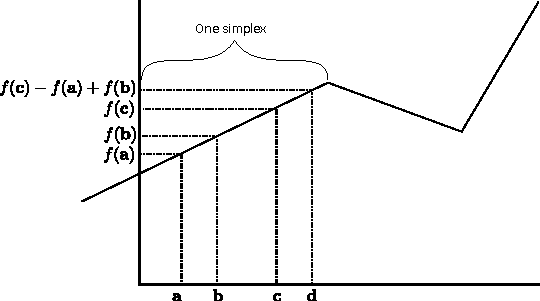
\includegraphics[width=3in]{figures/piecewise_affine.pdf}
  \caption{A real function $f$ that is piecewise affine.}
\label{FIG:piecewise_affine}
\end{figure}
The function $f$ is not affine, but is instead \textbf{piecewise affine}. We
know from our results that for any elements $\mathbf{a}, \mathbf{b},
\mathbf{c}, \mathbf{d} \in X^m$ that are on the same simplex (a simplex is here
defined as a subset of $X^m$ where $f$ is affine), then we can correctly
predict the value of $f(\mathbf{d})$ from those of $f(\mathbf{a}),
f(\mathbf{b}), f(\mathbf{c})$. Well in $\mathbb{R}^m$ this result is not really
useful, but we can actually show that every Boolean function is piecewise
affine! So theoretically, if we can identify all the simplices, this means that
we should be able to produce a sound extension in any case, for any function
$f$, and for any training set. At this point, only preliminary experiments
have been carried out, and a more thorough investigation deserves to be
performed.\\

Finally, we will close this discussion by opening to transfer learning.
Transfer learning is a current trend in the machine learning community, whose
purpose is to use the knowledge of a source problem $S$ to apply it to a less
known target problem $T$. Undoubtedly, transferring knowledge is the essence
of analogy. Current techniques in transfer learning usually involve statistical
tools (see e.g.  \cite{PanYanTKDE10} for a survey), and the use of analogical
proportions for such purposes is still entirely to be explored.

\newpage

\section*{Conclusion in French}

Les deux principaux objectifs de cette thèse étaient les suivants : exhiber des
propriétés théoriques des classifieurs analogiques, et appliquer le
raisonnement analogique au problème de la recommandation. Commençons par
rappeler succinctement les principaux résultats et contributions apportées dans
ce document (on ne suivra pas nécessairement l'ordre des chapitres).

\paragraph{Contributions\\}

Le premier chapitre était dévoué aux prérequis nécessaires sur les modèles de
raisonnement analogique existant, en accordant une attention particulière aux
modèles qui permettent l'implémentation de programmes informatiques. Dans le
deuxième chapitre, nous avons décrit en détail différentes définitions de
proportions analogiques, en insistant particulièrement sur les proportions
booléennes et arithmétiques. Nous avons essayé d'apporter au lecteurs quelques
intuitions géométriques sur les propriétés de ces proportions. Enfin, nous
avons considéré un problème de classification booléenne basique, qui nous a
permis d'introduire le processus de résolution d'équation analogique, ainsi que
le principe d'inférence analogique. Ce principe stipule que si l'on a
$a:b::c:d$, alors on devrait aussi avoir $f(a):f(b)::f(c):f(d)$, où $f(x)$
détermine la classe de $x$. Lorsque $f(d)$ est inconnu, on peut l'inférer à
partir des valeurs de $f(a), f(b)$ et $f(c)$ ce qui nous permet d'appliquer ce
type d'inférence à des tâches de classification ou des problèmes plus généraux
encore comme celui de la prédiction de notes.\\

La recommandation analogique fut l'objet des chapitres
\ref{CHAP:background_reco_systems} et \ref{CHAP:analogical_recommendation}.
Chapitre \ref{CHAP:background_reco_systems} était un chapitre de prérequis, où
nous avons clairement défini le problème de la prédiction de notes, et décrit
deux familles d'algorithmes (les méthodes par voisinage et par factorisation de
matrice) qui nous servent de base pour comparer nos algorithmes.

Nous avons ensuite développé dans le chapitre
\ref{CHAP:analogical_recommendation} un premier algorithme pour la prédiction
de notes  \cite{HugPraRicISMIS15}, fondé sur l'idée que si quatre utilisateurs
sont en proportion (c.a.d. que leurs notes respectives sont en proportion
géométrique), alors cela doit aussi être vrai pour un item que l'un des
utilisateurs n'a pas encore noté. Cette approche est directement inspirée des
travaux en classification analogique. Nos expériences ont montré que les
performances de ces algorithmes sont proches de celles des techniques par
voisinage, mais leur complexité cubique conduisent à des temps de calculs
prohibitifs.

Cela nous a conduit à considérer une autre approche pour la recommandation
analogique, qui ne repose pas sur la recherche de triplets d'utilisateurs.
Cette approche \cite{HugPraRicSerFuzzIEEE16} qui repose sur la notion de
``\textit{clones}'', prend en compte le fait que chaque utilisateur a une
appréciation bien particulière de l'échelle de note qui est utilisée. Nos
résultats montrent que le concept de clone est très important et qu'il est
primordial de l'intégrer d'une manière ou d'une autre dans un algorithme de
prédiction de notes. Il est cependant nécessaire de noter que ce type de biais
de les notes avait déjà été considéré dans de précédents travaux. Nous noterons
cependant que nos travaux sur les systèmes de recommandation nous ont conduit à
développer une bibliothèque Python \cite{Surprise} qui permet de facilement
tester et développer des algorithmes de prédiction de note.

Enfin, nous avons proposé un algorithme pour la fouille de proportions
analogiques dans des bases de données incomplètes \cite{HugPraRicSerLFA16}, en
nous inspirant fortement des travaux en fouille de règles d'associations. Nous
avons utilisé cet algorithme pour extraire des proportions analogiques entre
films dans la base de données MovieLens, qui était celle que nous utilisions
pour nos algorithmes de prédiction de note. Les résultats suggèrent qu'en fait,
les analogiques potentielles restent d'un intérêt relativement faible, en ceci
qu'elle mettaient généralement en jeu des items soit également appréciés, soit
également désapprouvés. En d'autre termes, les notes relatives aux différents
utilisateurs pour les quatre films d'une même proportion étaient souvent les
mêmes. Ceci nous permet de rétrospectivement interpréter les résultats modestes
de notre premier algorithme pour la prédiction de note, car cela suggère que
finalement, l'algorithme ne pouvait trouver que trop peu de bonnes proportions
pour produire des estimations de qualité.\\


Dans le chapitre \ref{CHAP:functional_definition}, nous avons décrit nos
contributions au problème de la classification analogique
\ref{CHAP:functional_definition}. Notre première contribution a été de proposer
une définition fonctionnelle des classifieurs analogiques, qui a a
particularité d'unifier les approches préexistantes. A partir de cette
définition, nous avons été capables de dériver différentes propriétés
théoriques. En particulier, nous avons montré que la VC-dimension des
classifieurs analogiques était infinie, et que leur taux d'erreur est
intimement lié à celui des algorithmes $k$-NN. En fait, notre définition
fonctionnelle établie clairement le lien qui relie la classification analogique
et la classification par plus-proches-voisins. Nous avons montré en effet que
la classification se traduit en deux étapes. La première étape consiste à
étendre l'ensemble d'apprentissage en ajoutant de nouveaux exemples dont la
classe est estimée en utilisant le principe d'inférence analogique. Ensuite,
sur la base de cette extension analogique, un algorithme $k$-NN est utilisé
pour classer le reste des éléments qui ne sont pas dans l'extension. Ce nouveau
point de vue est assez intéressant car il fait clairement intervenir deux des
principales caractéristiques des proportions analogiques, à savoir la
créativité et l'inférence.

Dans le chapitre \ref{CHAP:analogy_preserving_functions}, nous nous sommes
intéressés à une question qui découle naturellement des conclusions du chapitre
\ref{CHAP:functional_definition}: comment assurer que l'extension analogique
soit saine ? En d'autres termes, existe-t-il un critère qui nous permette
d'être sûr que les éléments de l'extension analogique sont correctement
classés ? Nous avons été capables de répondre à cette question  pour les
domaines booléens : l'extension analogique est parfaitement saine si (et
seulement si) la fonction booléenne $f$ qui détermine les labels est une
fonction affine. Nous avons étendu ces résultats aux domaines réels, et au cas
où les attributs ont des valeurs nominales. Cette série de travaux ouvre la
porte à divers pistes de recherches futures, que nous mentionnons maintenant.

\paragraph{Axes de recherches futures\\}

Dans la section \ref{SEC:approximate_ap_functions}, nous avons présenté le
concept de fonction approximativement AP (fonction qui préserve
approximativement l'analogie). En effet en pratique, il n'y a aucun moyen de
savoir si la fonction cible $f$ est vraiment affine. Ainsi, il est d'un intérêt
crucial d'obtenir des garanties statistiques relatives à la qualité de
l'extension analogique lorsque la fonction $f$ s'éloigne de l'ensemble des
fonctions affines. Un résultat comme le suivant serait très intéressant :

$$P(\omegasf \geq \eta) > 1 - \delta,$$
où $\eta \in [0, 1]$ et $\delta \in [0, \frac{1}{2}]$ sont des fonctions 
qui dépendent de $\varepsilon$ et de $\mid S \mid$. La valeur $\varepsilon$
indique que $f$ est $\varepsilon$-proche de l'ensemble des fonctions affines.
Pour le moment, nous nous intéressons à un problème un peu plus simple. On se
propose en effet de chercher une borne $\delta$ telle que :

$$P(\omegasf < 1) < \delta,$$
où $\delta$ est toujours fonction de $\varepsilon$.  En d'autres termes, on
cherche à borner la probabilité de l'événement ``\textit{$\esfs$ contient des
erreurs}''\\


Nous avons aussi remarqué lors de nos expérimentations que même lorsqu'une
fonction ne préserve pas du tout l'analogie, la qualité de l'extension
analogique peut tout de même être très bonne. Cela est du au fait que la
procédure de vote majoritaire permet parfois de contrebalancer les erreurs de
certains predicteurs. Il est clair qu'une compréhension profonde du rôle de ce
vote majoritaire reste une étape clef dans l'étude des classifieurs
analogiques.

Un autre axe de recherche possible serait de tirer partie du fait que toute
fonction booléenne est en fait affine par morceaux. Si l'on peut être sûr que
quatre éléments sont dans un domaine où $f$ est affine, alors on peut appliquer
de manière correct le principe d'inférence analogique. Pour l'instant, nous
n'avons mené que des expérimentations très préliminaires  à ce sujet.\\

Enfin, nous terminerons cette discussion en évoquant l'apprentissage par
transfert (\textit{transfer learning}). L'apprentissage par transfert est un
sujet assez populaire de nos jours dans la communauté de l'apprentissage
artificiel, dont le but est de transférer des connaissances d'un problème
source $S$ pour les appliquer à un problème moins bien connu $T$.
Indubitablement, l'essence même de l'analogie est d'opérer un transfert de
connaissance. L'usage des proportions analogiques à un tel domaine
d'application reste encore entièrement à explorer.

